\documentclass[10pt,journal,compsoc]{IEEEtran}

\usepackage{algorithmic}
\usepackage{array}
\usepackage[nocompress]{cite}
\usepackage{color}
\usepackage{listings}
\usepackage[caption=false,font=normalsize,labelfont=sf,textfont=sf]{subfig}
\usepackage{stfloats}
\usepackage{url}
\usepackage{multirow}

\definecolor{lightgray}{rgb}{0.95,0.95,0.95}

\usepackage{listings}
\lstset{
    aboveskip=20pt,
    belowskip=20pt,
    lineskip=5pt,
    backgroundcolor=\color{white},
    basicstyle=\footnotesize\ttfamily,
    breakatwhitespace=true,
    breaklines=true,
    captionpos=b,
    extendedchars=true,
    frame=none,
    keepspaces=true,
    morekeywords={*,...},
    numbers=none,
    numbersep=5pt,
    rulecolor=\color{black},
    showspaces=false,
    showstringspaces=false,
    showtabs=false,
    stepnumber=2,
    tabsize=2,
    title=\lstname,
}

\usepackage[pdftex]{graphicx}
\graphicspath{{./figs}}
\DeclareGraphicsExtensions{.pdf,.jpeg,.png}


% *** MATH PACKAGES ***
\usepackage{amsmath}
\interdisplaylinepenalty=2500

% correct bad hyphenation here
\hyphenation{op-tical net-works semi-conduc-tor}

\begin{document}

% title
\title{Reproducible Workflow on a Public Cloud for Computational Fluid Dynamics}
% author names and affiliations
\author{Olivier Mesnard, Lorena A. Barba
\IEEEcompsocitemizethanks{\IEEEcompsocthanksitem Mechanical and Aerospace Engineering,
the George Washington University, Washington, DC 20052.\protect\\
% note need leading \protect in front of \\ to get a newline within \thanks as
% \\ is fragile and will error, could use \hfil\break instead.
E-mail: mesnardo@gwu.edu
\IEEEcompsocthanksitem Email: labarba@gwu.edu}% <-this % stops an unwanted space
%\thanks{Manuscript submitted 2019}
}

\IEEEtitleabstractindextext{%
\begin{abstract}
In a new effort to make our research transparent and reproducible by others, we developed a workflow to run computational studies on a public cloud. It uses Docker containers to create an image of the application software stack. We also adopt several tools that facilitate creating and managing virtual machines with compute nodes and submitting jobs to these nodes. The configuration files for these tools are part of an expanded "reproducibility package" that includes workflow definitions for cloud computing, in addition to input files and instructions. This facilitates re-creating the cloud environment to re-un the simulations under the same conditions.
\end{abstract}
}

% make the title area
\maketitle

\IEEEraisesectionheading{\section{Introduction}\label{sec:introduction}}

Reproducible research and replication studies are essential components for the progress of evidence-based science, even more now when nearly all fields advance via computation.
We use computer simulations and data models to create new knowledge,
but how do we provide evidence that this new knowledge is justified? 
Traditional journal publications exclude software and data products from the peer-review process, yet reliance on ever more complex computational artifacts and methods is the norm.
Lacking standards for documenting, reporting and reviewing the computational facets of research, it becomes difficult to verify and corroborate the findings presented in journals and conferences \cite{donoho_et_al_2009}.

The literature is cluttered with confused and sometimes contradictory definitions for reproducible research, reproducibility, replicability, repetition, etc.\cite{barba_2018}.
It is thus worth clarifying how we use these terms.
``Reproducible research'' was used by geophysics professor Jon Claerbout in the 1990s to mean computational studies that can be reproduced by other scientists. His research group at Stanford created a reproducible-research environment\cite{schwab_et_al_2000} whose goal was complete documentation of scientific computations, in such a way that a reader could reproduce all the results and figures in a paper using the author-provided computer programs and raw data.
This requires open data and open source software and, for this reason, the reproducibility movement is closely linked with the open science movement.
The term ``replication'' has been adopted to refer to an independent study generating new data which, when analyzed, lead to the same findings \cite{peng_2011}.
We follow this convention, adopted also recently in a report from the National Academies of Sciences, Engineering, and Medicine \cite{nasa_oss_2018}.

Many efforts to develop cyberinfrastructure that supports reproducible research have been launched in past years. 
They address concerns like automatic capture of changes to software (version control systems), persistent data archival, global registration of data identifiers, workflow management, and more. 
But capturing the whole computational environment used in a research project remains one of the most difficult problems. 
Computational researchers often use a multi-layer stack of software applications that can be laborious to build from scratch. 
Container technology like Docker is a recent addition to the reproducibility toolbox \cite{boettiger_2015}. 
In this work, we develop and assess a workflow for reproducible research on a public cloud, adopting Docker containers and several other tools to automate and fully document scientific computations.

Universities and national laboratories spend millions of dollars to deploy and maintain on-site high-performance computing (HPC) clusters.
At the George Washington University, we have access to a university-managed HPC cluster called Colonial One.
The cluster is now $6$ years old and approaching its end-of-life.
On average, its computational resources are idle $9\%$ of the time and unavailable to users for roughly 5 days a year (due to maintenance).
Administrators of the cluster have been recently considering integrating cloud-computing platforms in the research-computing portfolio. 
Over the past decade, cloud-computing platforms have rapidly evolved, now offering solutions for scientific applications.
From a user's point of view, a cloud platform offers great flexibility (hardware and virtual machines) with instantaneous availability of infinite (in appearance) computational resources.
No more waiting time in job-submission queues!
This promises to greatly facilitate code development, debugging, and testing. Resources allocated on the cloud are released as soon as the job is done, avoiding paying for idle time.
On a public-cloud platform with a "pay-as-you-go" type of subscription---such as Microsoft Azure, Google Cloud, Amazon AWS---a user directly sees how much it costs to run a scientific application, while such information usually remains obscure to the end-user on university-managed clusters. 
Cost models that make sense for researchers, labs, and universities are still unclear. 
Yet, this information is key when making a decision to adopt a cloud workflow for research. 
We report here what we have learned from nearly two years of using cloud computing for our simulation-based workflow, with the hope that it will shed some light on the costs and benefits, and help others considering using cloud computing for their research.

\section{Reproducible cloud-based workflow}\label{sec:workflow}

Scientific publications reporting computational results often lack sufficient details to reproduce the researcher's computational environment; e.g., they may miss to mention external libraries used along with the main computational code.
We have learned the hard way how even different versions of the same external library can alter the numerical results and even the scientific findings of a computational study\cite{mesnard_barba_2017}.
This section presents an overview and mini-tutorial of the workflow we developed to guarantee the highest level of reproducibility of our computational research, with the best available technology solutions. 
In the process of creating this reproducible workflow, we also evaluated the suitability of public cloud offerings by Microsoft Azure for our research computing needs. 
The tools we adopted for computing on cloud resources are specific for this provider. 

\subsection{Use of container technology}

\begin{figure*}
    \begin{center}
        \colorbox{lightgray}{
        \begin{minipage}[c]{14cm}
        \bigskip
        \small \sffamily{
        \subsection*{Docker Terminologies:}
{\sf \footnotesize
\textbf{Docker}--- An open source OS-level virtualization software to create and run multiple independent, isolated, and portable containers on the same host Operating System.\\
\vspace{0.1cm}\\
\textbf{Docker Image}--- Union of layered filesystems stacked on top of each other. Each layer defines a set of differences from the previous layer. A user composes (builds) a Docker image using a \texttt{Dockerfile}, usually starting from a base image (such as \texttt{ubuntu:16.04}).\\
\vspace{0.1cm}\\
\textbf{Docker Container}--- A standardized unit created from a Docker image to deploy an application or a runtime environment. A Docker container can be seen as an instance of a Docker image that includes an additional writable layer at the top of the layered stack. When a container is deleted, so is the writable layer, while the image remains unchanged.\\
\vspace{0.1cm}\\
\textbf{Dockerfile}--- An ASCII file including the sequence of instructions to create a Docker image for the computational runtime environment. A Dockerfile contains Docker keywords such as \texttt{FROM}, \texttt{RUN}, or \texttt{COPY}. Each instructions in the \texttt{Dockerfile} creates a layer in the Docker image.\\
\vspace{0.1cm}\\
\textbf{DockerHub}--- The official registry of Docker Inc.; a cloud-based registry service to store, share, and retrieve (public or private) Docker images.\\
}}
        \vspace{0.2cm}
        \end{minipage}}
    \end{center}
\end{figure*}

To overcome the so-called ``dependency hell'' and facilitate reproducibility and portability, we use the container technology provided by the open-source project Docker.
A container represents an isolated user space where application programs run directly on the operating system's kernel (with limited access to its resources).
In contrast with virtual machines, containers do not include a full operating system, making them lighter and faster.
Containers allow re-creating the same runtime environment of an application (including all its dependencies) from one machine to another. 
They empower researchers to share pre-built images of their software stack, ameliorating one of the biggest pain points for reproducible research: building the software in a different machine. 
The majority of enterprise developers today are familiar with Docker container technology (first released six years ago). 
But in academic settings, many are still unaware of its value. 
We present this section as an overview for research software developers unfamiliar with Docker, but comfortable with scripting, version control, and distributed collaboration.

A container is an instance of an image.
The developer builds this image on a local machine and pushes it to a public registry to share it with other users.
Users pull the image from the public registry,---in our case, DockerHub---and create containers out of it.
To create a Docker image, the developer writes a \texttt{Dockerfile}.: an ASCII file containing commands that tell Docker what to do.
For example, we create a new image from a base image using the keyword \texttt{FROM}.
We then write the different commands to build a multi-layered runtime environment of the application that includes all its dependencies.
Once we have built the image on the local machine, we push it to a repository on the DockerHub registry: a place to store and retrieve Docker images.
Listing \ref{lst:docker_build_push} provides the command lines to build (\texttt{docker build}) and push (\texttt{docker push}) an image of our CFD software (\texttt{barbagroup/petibm:0.4-GPU-IntelMPI-ubuntu}) that we used to obtain some of the results presented in the next section.
Here, \texttt{CLOUDREPRO} is an environment variable set to the local path of the GitHub repository for this paper, \texttt{cloud-repro}\footnote{\url{https://github.com/barbargroup/cloud-repro}} cloned on the user's machine.

\begin{lstlisting}[label=lst:docker_build_push,caption={Build and push a Docker image.}]
$ cd $CLOUDREPRO/docker/petibm
$ docker build --tag=barbagroup/petibm:0.4-GPU-IntelMPI-ubuntu --file=Dockerfile .
$ docker push barbagroup/petibm:0.4-GPU-IntelMPI-ubuntu
\end{lstlisting}

\noindent Anyone can now pull the application image from DockerHub, and create a Docker container to run the CFD application software in a faithfully reproduced local environment.
The great advantage of container technology is that the same container that was built and tested on the developer's local machine can now run at scale in production mode on virtual machines, bare metal, or even cloud platforms.
Our objective is to create and run containers on a public cloud provider such as Microsoft Azure.
Figure \ref{fig:cloud_workflow} shows a graphical representation of the workflow we developed using Docker and various tools for running CFD simulations on Microsoft Azure.
The next section explains these tools. 

\subsection{Use of public cloud resources}

To run computational jobs on Microsoft Azure, we use several tools that facilitate creating and managing virtual machines with compute nodes, and submitting jobs to those nodes.
We use a service called Azure Batch that leverages Microsoft Azure at no extra cost, relieving the user from manually creating, configuring, and managing an HPC-capable cluster of cloud nodes, including virtual machines, virtual networks, job and task scheduling infrastructure.
Azure Batch works with both embarrassingly parallel workloads and tightly-coupled MPI jobs (the latter being the case of our CFD software).
To use Azure Batch, we first need to configure a workspace on Microsoft Azure.
This can be done either via the Azure Portal in a web browser or from a local terminal using the open-source tool Azure CLI.\footnote{Azure CLI (version 2.0.57): \url{https://github.com/Azure/azure-cli}}
We prefer to use the command-line solution (program \texttt{az}), as it allows us to keep track of the steps done to configure the Azure workspace (see Listing \ref{lst:az_configure}).
First, we set the subscription we want to use (let's call it \texttt{reprosubscription}).
Next, we create a resource group, \texttt{reprorg}, located in this case in the East US region, which will contain all the Azure resources.
We create an Azure Storage account, \texttt{reprostorage}, in the resource group,
and we also need to create an Azure Batch account, \texttt{reprobatch} and associate it to the storage account.
Finally, we create a fileshare (of size $100$ Gb) in the storage.

\begin{lstlisting}[label=lst:az_configure,caption={Configure the workspace on Microsoft Azure.}]
$ az account set --subscription reprosubscription
$ az group create --name reprorg --location eastus
$ az storage account create --name reprostorage --resource-group reprorg --sku Standard_LRS --location eastus
$ az batch account create --name reprobatch --resource-group reprorg --location eastus --storage-account reprostorage
$ az storage share create --name fileshare --account-name reprostorage --account-key storagekey --quota 100
\end{lstlisting}

To create computational nodes and submit container-based jobs to Azure Batch, we use the open-source command-line utility Batch Shipyard.\footnote{Batch Shipyard (version 3.6.1): https://github.com/Azure/batch-shipyard}
Batch Shipyard is entirely driven by configuration files: the utility parses user-written YAML files to automatically create pools of compute nodes on Azure Batch and to submit jobs to those pools.
Typically, we need to provide four configuration files:

\begin{itemize}
    \item \texttt{config.yaml} contains information about the Azure Storage account and Docker images to use.
    \item \texttt{credentials.yaml} stores the necessary credentials to use the different Microsoft Azure service platforms (e.g., Azure Batch and Azure Storage).
    \item \texttt{pool.yaml} is where the user configures the pool of virtual machines to create.
    \item \texttt{jobs.yaml} details the configuration of the jobs to submit to the pool.
\end{itemize}

Once the configuration files are written, we invoke Batch Shipyard through the \texttt{shipyard} program on our local machine.
The folder \texttt{examples/snake2d2k35/config\_shipyard} in the repository accompanying this paper contains an example YAML files to create a pool of two \texttt{NC24r} compute nodes (featuring K80 GPUs and InfiniBand network).
Listing \ref{lst:shipyard_run} shows the commands to run from your local terminal to create a pool of compute nodes on Azure Batch and submit jobs to it.
During the pool creation (\texttt{shipyard pool add}), the Docker image of our CFD application is pulled from the registry to the virtual machines.
With \texttt{shipyard data ingress}, we can upload input files to the compute nodes.
Once created, we submit jobs to the pool (\texttt{shipyard jobs add}); the tasks for a job will start automatically.

\begin{lstlisting}[label=lst:shipyard_run,caption={Create a pool with Batch Shipyard and submit jobs to it.}]
$ cd $CLOUDREPRO/examples/snake2d2k35
$ az storage directory create --name snake2d2k35 --share-name fileshare --account-name reprostorage
$ export SHIPYARD_CONFIGDIR=config_shipyard
$ shipyard pool add
$ shipyard data ingress
$ shipyard jobs add
\end{lstlisting}

Once the simulations are done (i.e., the job tasks are complete), we delete the jobs and the pool (Listing \ref{lst:shipyard_del}).
The output of the computation is now stored in the fileshare in our Azure Storage account.
We can download the data to our local machine to perform additional post-processing steps.

\begin{lstlisting}[label=lst:shipyard_del,caption={Delete the pool and jobs, and download to output to a local machine.}]
$ shipyard pool del
$ shipyard jobs del
$ mkdir output
$ az storage file download-batch --source fileshare/snake2d2k25 --destination output --account-name reprostorage
\end{lstlisting}

Reproducible research requires authors to make their code and data available.
Thus, the Dockerfile and YAML configuration files should be made part of an extended reproducibility package that includes workflow instructions for cloud computing, in addition to other input files.
Such reproducibility package facilitates re-creating the cloud environment to run the simulations under the same conditions.
The reproducibility packages of the examples showcased in the next section are available in the GitHub repository \texttt{cloud-repro}, which includes instructions on how to reproduce the results.

\begin{figure*}[!h]
    \centering
    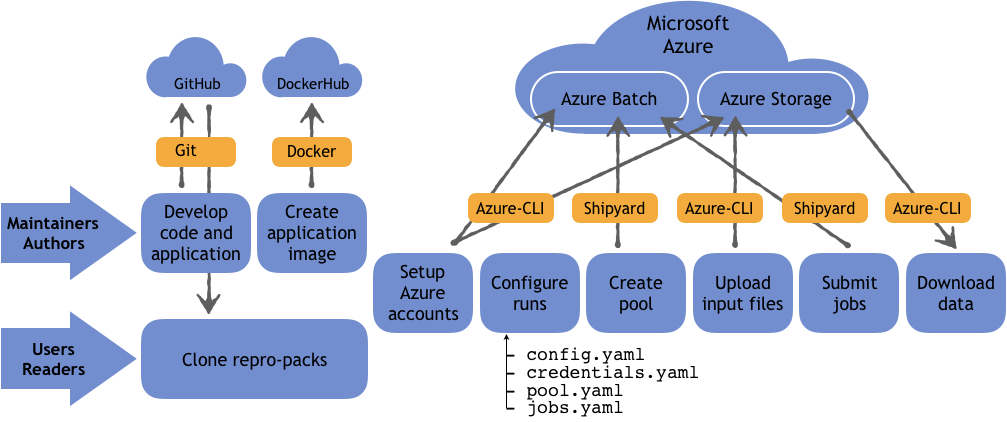
\includegraphics[width=16cm]{figures/cloud_workflow.png}
    \caption{Reproducible workflow on the public cloud provider Microsoft Azure. Our CFD software is version-controlled with Git and GitHub. We push to DockerHub a Docker image of our CFD application with all its dependencies. Azure-CLI is use to configure accounts on Microsof Azure and to upload/download data to/from an Azure Storage account. With Batch Shipyard, we can create pool on Azure Batch and run container-based simulation using our Docker image.}
    \label{fig:cloud_workflow}
\end{figure*}

\section{Results}\label{sec:results}

The top concerns of researchers considering cloud computing are performance and cost. 
Until just a few years ago, the products offered by cloud providers were unsuitable to the needs of computational scientists using HPC, due to performance overhead of virtualization and lack of support for fast networking. 
Azure only introduced nodes with GPU devices and Infiniband support in 2017. 
Our first objective was to assess performance on cloud nodes for the type of computations in our research workflows with  tightly coupled parallel applications. 
We present results from benchmarks and test-cases showing that we are able to obtain similar performance in terms of latency and bandwidth using the Azure virtual network, comparing to a traditional university-managed HPC cluster (Colonial One).
Table \ref{tab:hw_specs} lists the hardware specifications of the nodes used on Microsoft Azure and Colonial One.
 Our target research application relies on three-dimensional CFD simulations with our in-house research software. We include here a sample of the types of results needed to answer our research question, obtained by running on the public cloud using the reproducible workflow described in Section \ref{sec:workflow}. 
 The goal is to showcase the potential of cloud computing for CFD, share the lessons we learned in the process, as well as analyze the cost scenarios for full applications.


\begin{table*}[b]
    \renewcommand{\arraystretch}{1.5}
    \caption{Hardware Specifications of Nodes Used on Microsoft Azure and Colonial One. On Both Platforms, MPI Applications Take Advantage of RDMA (Remote Direct Memory Access) Network with FDR InfiniBand.}
    \label{tab:hw_specs}
    \centering
    \begin{tabular}{cccccccc}
        Platform & Node & Intel Xeon CPU & \# threads & NVIDIA GPU & RAM (GiB) & SSD Storage (GiB) \\
        \hline
        \multirow{2}{*}{Azure} & \texttt{NC24r} & Dual 12-Core E5-2690v3 (2.60GHz) & 24 & 4 x K80 & 224 & 1440 \\
        & \texttt{H16r} & Dual 8-Core E5-2667v3 (3.20GHz) & 16 & - & 112 & 2000 \\
        \hline
        \multirow{2}{*}{Colonial One} & \texttt{Ivygpu} & Dual 6-Core E5-2620v2 (2.10GHz) & 12 & 2 x K20 & 120 & 93 \\
        & \texttt{Short} & Dual 8-Core E5-2650v2 (2.60GHz) & 16 & - & 120 & 93 \\
        \hline
    \end{tabular}
\end{table*}

\subsection{MPI Communication Benchmarks}\label{subsec:mpi_benchmarks}

Point-to-point MPI benchmarks from the Ohio State University Micro-Benchmarks\footnote{OSU Micro-Benchmarks (version 5.6): \url{http://mvapich.cse.ohio-state.edu/benchmarks/}} suite ran on Microsoft Azure and Colonial One to investigate performance in terms the latency and bandwidth.
The latency test is carried out in a ping-pong fashion and measures the time elapsed to get a response; the sender sends a message with a certain data size and wait for the receiver to send back the message with the same data size.
The bandwidth test measures the maximum sustained rate that can be achieved on the network; it consists in having the sender sends a fixed number of messages to a receiver that replies only after receiving all of them.
The tests ran on \texttt{NC24r} nodes on Azure and \texttt{Ivygpu} nodes on Colonial One, all them featuring a network interface for RDMA (Remote Direct Memory Access) connectivity to communicate over an InfiniBand network.
Fig. \ref{fig:osu_benchmarks} reports the mean latencies and bandwidths obtained over $5$ repetitions on both platforms.

\begin{figure}[!h]
    \centering
    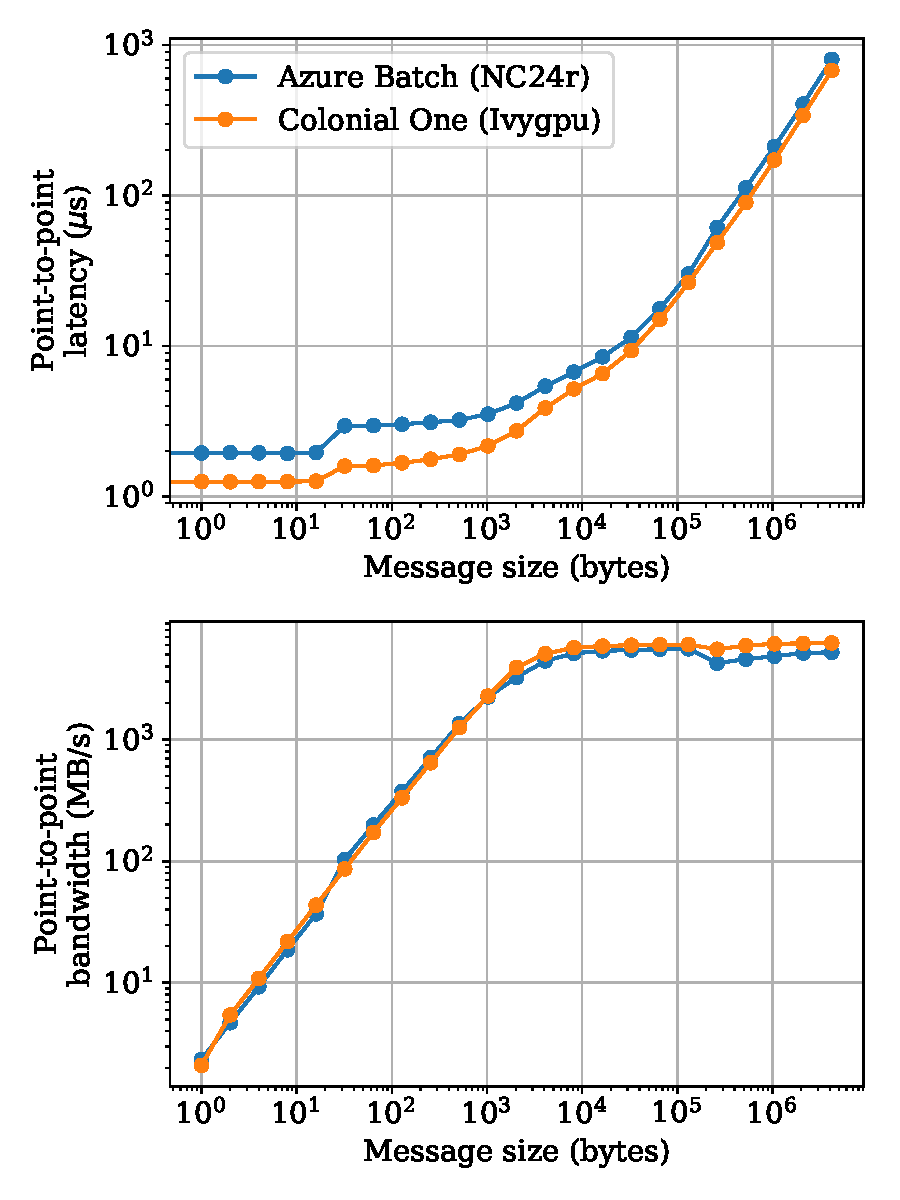
\includegraphics[width=8cm]{figures/osu_latency_bandwidth.pdf}
    \caption{Point-to-point latency (top) and bandwidth (bottom) obtained on Colonial One (\texttt{Ivygpu} nodes) and on Microsoft Azure (\texttt{NC24r} nodes). Benchmark results are averaged over $5$ repetitions.}
    \label{fig:osu_benchmarks}
\end{figure}

\subsection{Poisson Benchmarks}\label{subsec:poisson_benchmarks}

CFD algorithms often require to solve linear systems with iterative methods.
For example, the project method implemented in our research software solve a Poisson system every time step to project the velocity field onto the divergence-free space (to satisfy the incompressibility constraint).
Thus, we investigated the time-to-solution to solve a three-dimensional Poisson system (obtained with a 7-point stencil using central differences) on different nodes of Microsoft Azure and Colonial One.
The system was solved using a Conjugate-Gradient (CG) method with a classical Algebraic MultiGrid (AMG) preconditioner with an exit criterion set to an absolute tolerance of $10^{-12}$.
The iterative solver ran on CPU nodes (\texttt{H16r} instances on Azure and \texttt{Short} nodes on Colonial One) using the CG algorithm from the PETSc library\cite{balay_et_al_2018} and an AMG preconditioner from Hypre BoomerAMG.
Fig. \ref{fig:poisson_benchmarks} (top) reports the mean runtimes (averaged over $5$ repetitions) to iteratively solve the system, on a uniform grid of $50$ million cells ($1000 \times 1000 \times 50$), as we increase the number of nodes in the pool.
We also solved the Poisson system with the NVIDIA AmgX library on multiple GPU devices using \texttt{NC24r} instances on Azure and \texttt{Ivygpu} nodes on Colonial One.
The Poisson system for a base mesh of $6.25$ million cells ($500 \times 500 \times 25$) is solved on a single node using $12$ MPI processes and $2$ GPU devices; we then double the mesh size as we double the number of nodes.
As the number of iterations to reach convergence increases with the size of the system, we normalize the runtimes by the number of iterations.
Fig. \ref{fig:poisson_benchmarks} (bottom left) shows the normalized mean runtimes ($5$ repetitions) obtained on Azure and Colonial One.
The bottom-right panel of the figure reports the normalized mean runtimes obtained on Azure when we put more constraint on the bandwidth; the base mesh now contains $25$ millions cells ($1000 \times 500 \times 50$).

\begin{figure}[!h]
    \centering
    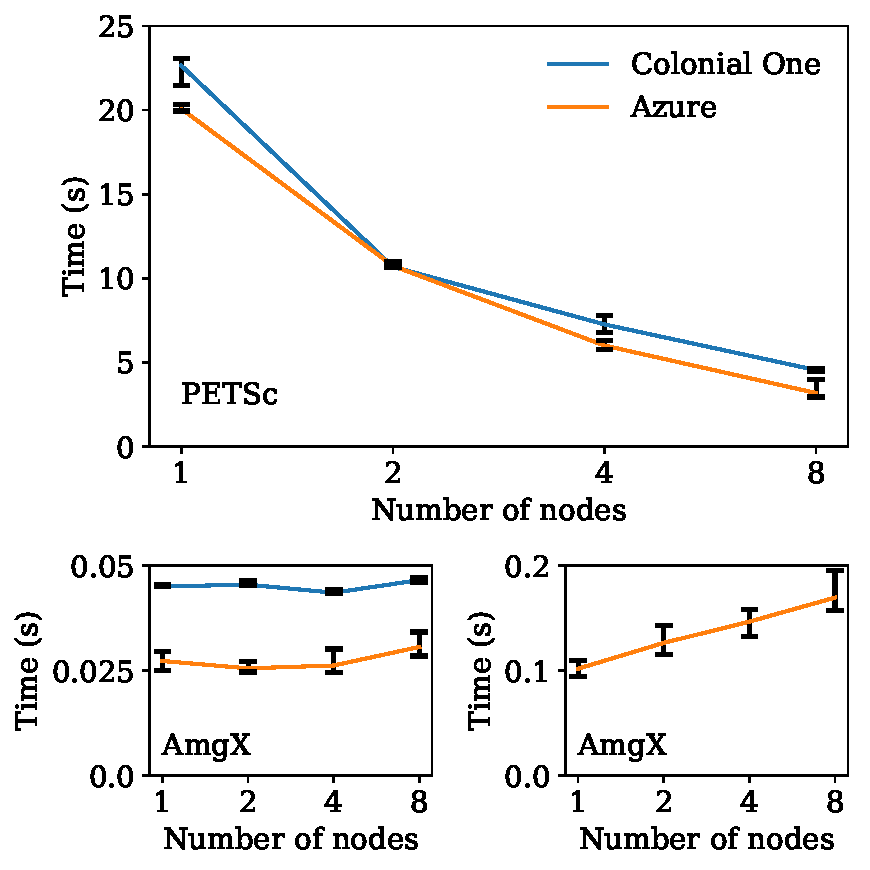
\includegraphics[width=8cm]{figures/poisson_time_vs_nodes.pdf}
    \caption{Runtimes to solve a Poisson system on Colonial One and on Microsoft Azure. Benchmark was repeated 5 times and we report the mean runtimes as well as the extrema. Poisson system was solved on Azure using PETSc on \texttt{H16r} nodes and using AmgX on \texttt{NC24r} nodes. On Colonial One, we solved the system with PETSc on \texttt{Short} nodes and with AmgX on \texttt{Ivygpu} nodes. The runs with PETSc solved a Poisson system on a mesh size of 50 million cells (top). With AmgX (bottom left), the base mesh size contains 6.25 million cells and we scale it with the number of nodes. On Azure, we also ran the Poisson benchmark with a finer base mesh size of 25 million cells (bottom right). Runtimes obtained with AmgX were normalized by the number of iterations required to reach a absolute tolerance of $10^{-12}$.}
    \label{fig:poisson_benchmarks}
\end{figure}

\subsection{Flow Around a Flying Snake Cross-Section}\label{subsec:snake}

Our research lab is interested in understanding the aerodynamics of flying animals using Computational Fluid Dynamics software.
One of our applications deals with the aerodynamics of a snake species, \textit{Chrysopelea Paradisi}, that lives in South-East Asia.
The arboreal reptile has the remarkable capacity to turn its entire body into a wing and glide over several meters\cite{socha_2011}.
The so-called flying snake jumps from tree branches, undulates in the air, and is able to produce lift by expanding its ribcage to flatten its ventral surface (morphing its normally circular cross-section into a triangular shape).

To study the flow around the flying snake, we develop a in-house CFD software called PetIBM\cite{chuang_et_al_2018}, a open-source toolbox that solves the two- and three-dimensional incompressible Navier-Stokes equations using a projection method (an approximate block-LU decomposition of the fully discretized equations\cite{perot_1993}) and an Immersed-Boundary Method (IBM).
Within this framework, the fluid equations are solved on a extended grid that does not conform to the surface of the immersed body.
To model the presence of the body, the momentum equation is augmented with a forcing term that is activated in the vicinity of the immersed boundary.
This technique allows the use of simple fixed structured Cartesian grids to solve the equations.
PetIBM also implements Immersed Boundary Methods (IBMs) that fit into the projection method and, in the present study, we use an implementation of the IBM proposed in \cite{li_et_al_2016}.
PetIBM runs on distributed-memory architectures and relies on the efficient data structures and parallel routines of the PETSc library.
The software also implements the possibility to solve linear systems on multiple GPU devices distributed across the nodes with the NVIDIA AmgX and AmgXWrapper\cite{chuang_barba_2017}.
To obtain reproducible computational results, the code used to run the simulations needs to be made available.
In that regard, PetIBM is open source, version-controlled on GitHub,\footnote{PetIBM (version 0.4): \url{https://github.com/barbagroup/PetIBM}} and developed under the permissive BSD-3 clause license.

\subsubsection{2D Flow Around a Snake Cross-Section}

With Batch Shipyard, we submitted a job on Azure Batch to compute the two-dimensional flow around an anatomically accurate sectional shape of the gliding snake.
The cross-section has a chord-length of $1$ and forms a $35$-degree angle of attack with the incoming freestream flow.
The Reynolds number, based on the freestream speed, the body chord-length, the kinematic viscosity, is set to $Re=2000$.
The immersed boundary is centered in a $30c \times 30c$ computational domain that contains just above $2.9$ million cells.
The grid is kept uniform with the highest resolution in the vicinity of the body and stretched to the external boundaries with a constant ratio (see Table \ref{tab:grid_specs} for details about the grid).
(The immersed boundary is discretized with the same resolution than the background fluid grid.)
A convective condition was used at the outlet boundary while freestream conditions were enforced on the others.
The job was submitted to a pool of two \texttt{NC24r} nodes, with $12$ MPI processes and $2$ GPU devices per node.
The task completed $200,000$ time steps (i.e., $80$ time units of flow simulation with a time-step size $\Delta t = 0.0004 c / U_\infty$) in just above $7$ hours.

Fig. \ref{fig:force_coefficients} shows the history of the force coefficients on the two-dimensional cross-section.
The lift coefficient only maintains its maximum mean value during the early stage of the simulation (up to $40$ time units).
Between $40$ and $50$ time units, the mean value starts to drop.
The time-averaged force coefficients (between $40$ and $80$ time units) are reported in Table \ref{tab:force_coefficients}.
Fig. \ref{fig:wz_2d} shows snapshots of the vorticity field after $20$, $44$, $45$, and $80$ time unit of flow simulation.
After $20$ time units, the vortices shed from the snake section are almost aligned in the near wake (with a slight deflection towards the lower part of the domain).
Snapshots of the vorticity at time units $44$ and $45$ show that the initial alignment is perturbed by vortex-merging events (same-sign vortices merging together to form a stronger one).
Following that, the wake signature is altered for the rest of the simulation: vortices are not aligned anymore, the wake becomes wider (leading to lower aerodynamic forces) with a 1S+1P vortex signature (a single clockwise-rotating vortex on the upper part and a vortex pair on the lower part).

\begin{figure}[!h]
    \centering
    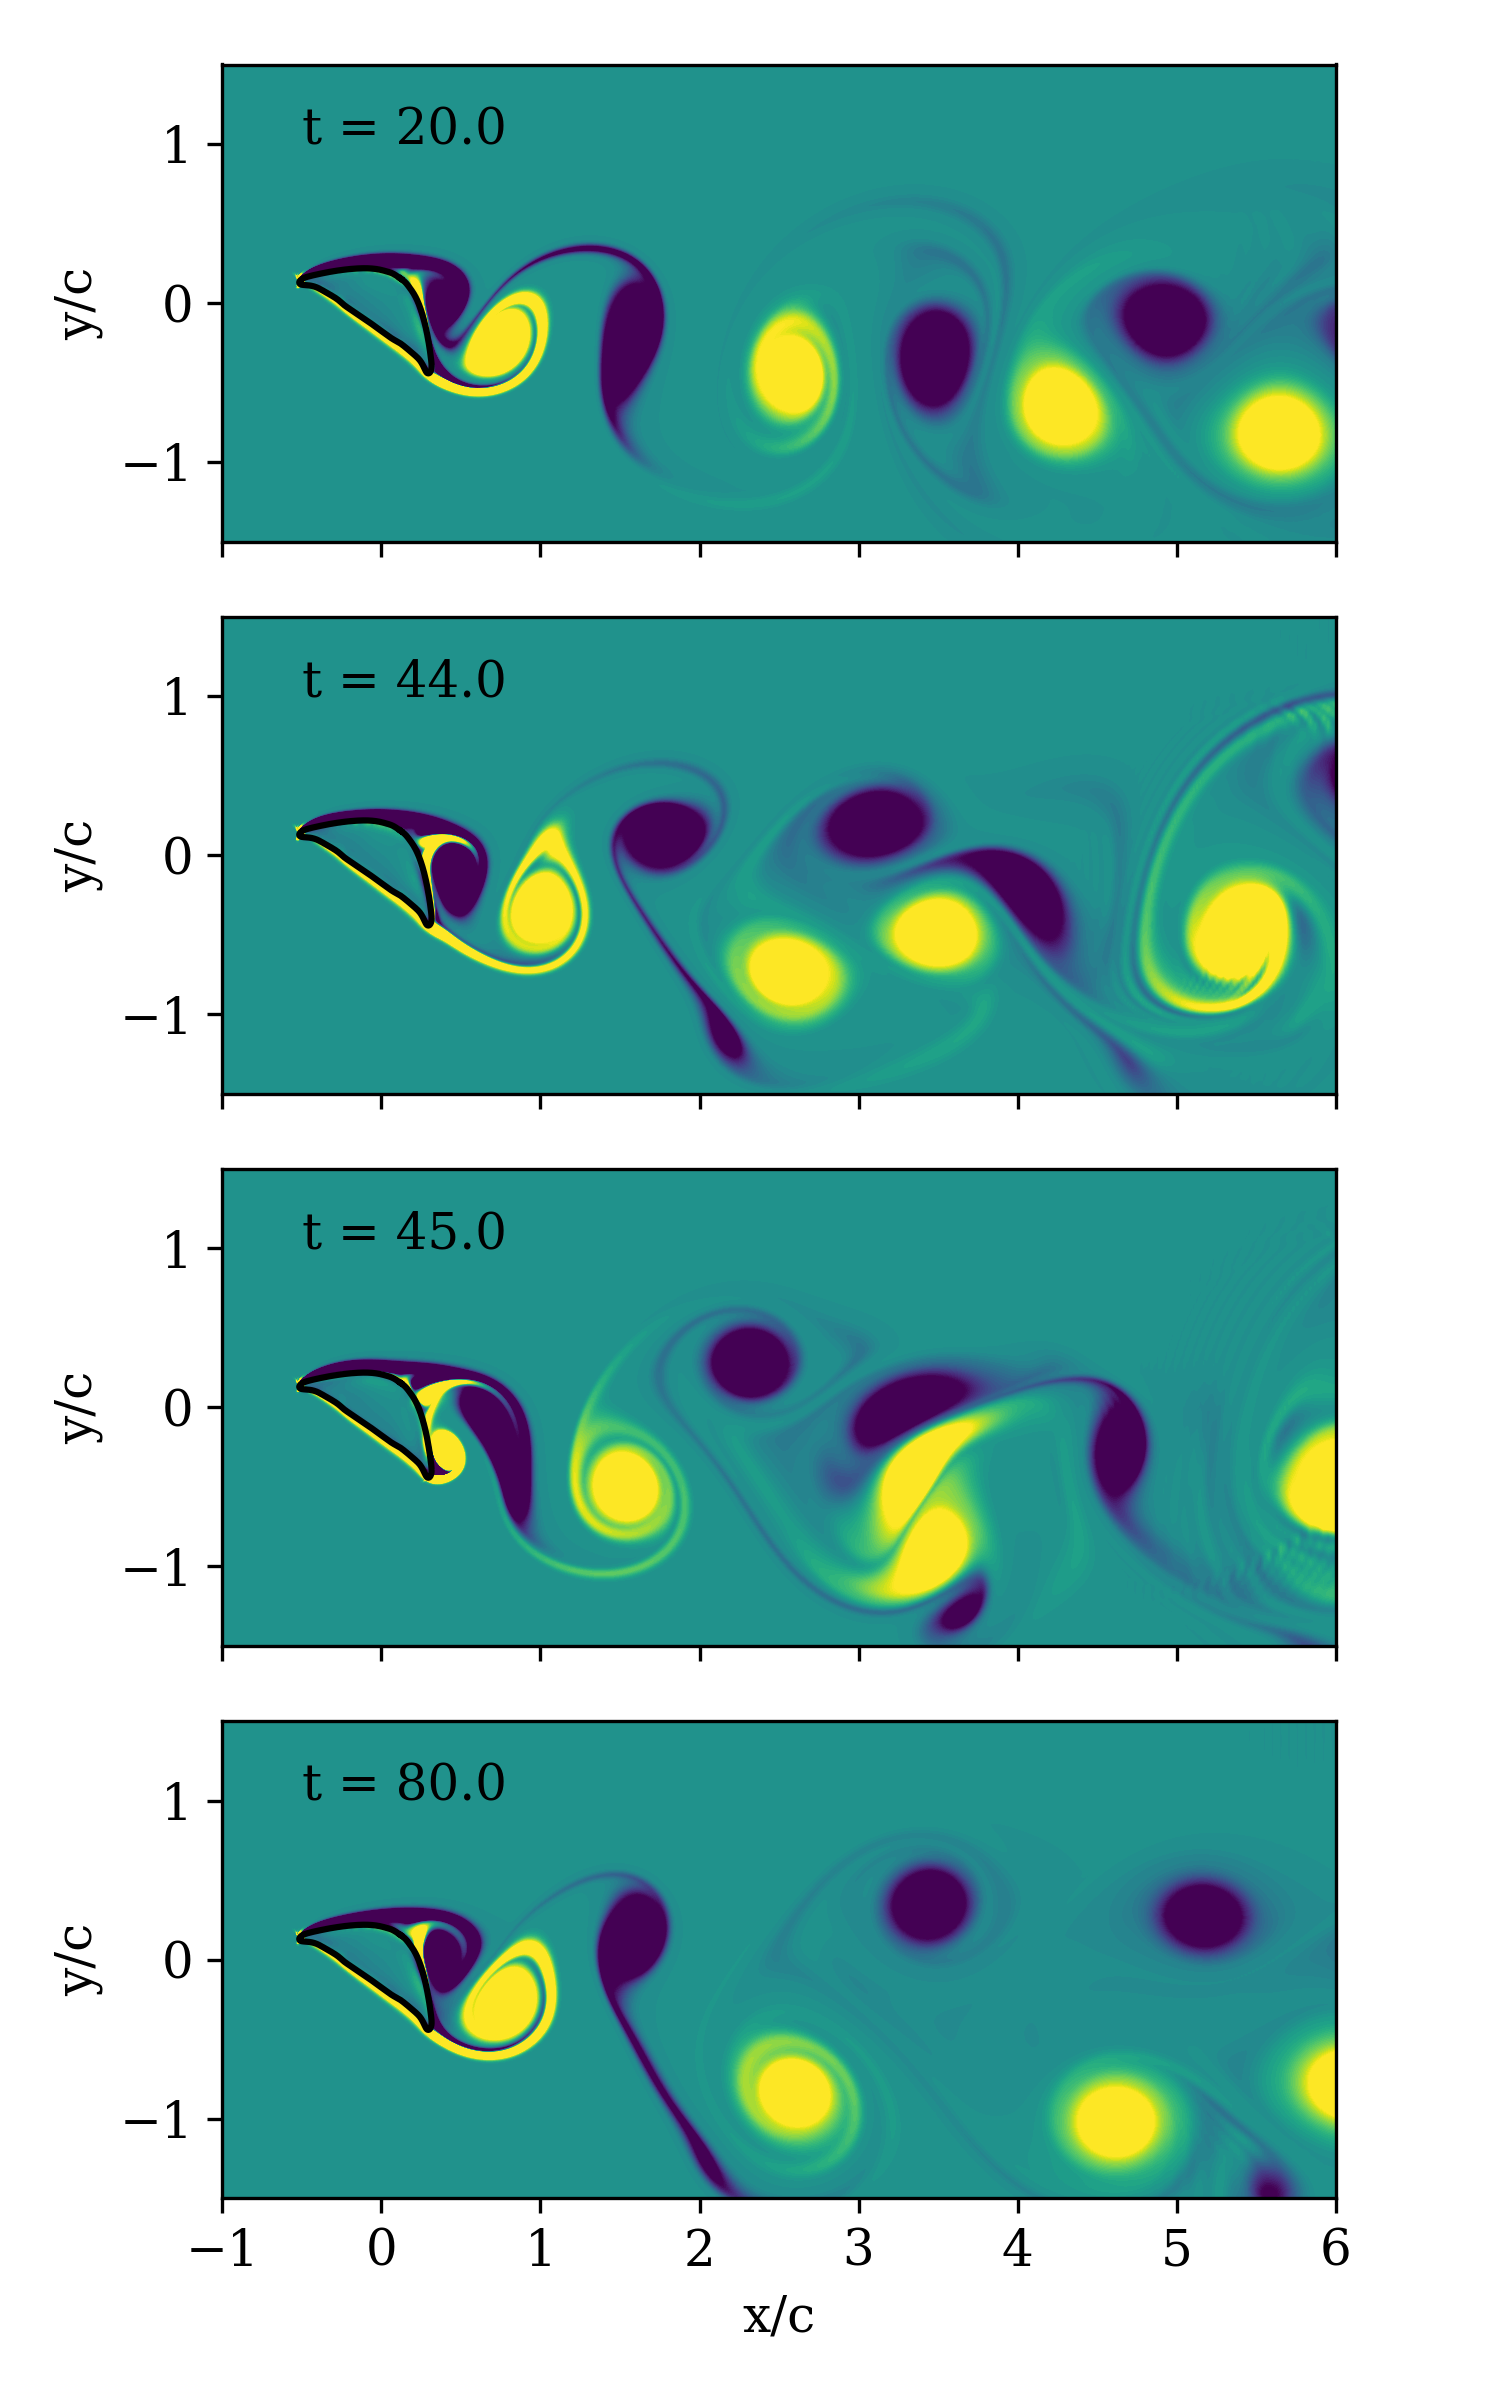
\includegraphics[width=8cm]{figures/wz_multi_contourf.png}
    \caption{Filled contour of the vorticity field ($-5 \leq w_z c / U_\infty \leq 5$) after $20$, $44$, $45$, and $80$ time units of flow simulation with PetIBM for the snake cross-section at a $35$-degree angle of attack and Reynolds number $2000$. Vortex merging events are responsible for the change in the wake signature and the drop in the mean value of the lift coefficient.}
    \label{fig:wz_2d}
\end{figure}

\subsubsection{3D Flow Around a Snake Cylinder}

Although the two-dimensional simulations gave us some insights into to flow dynamics happening in the behind the snake, we know that at this Reynolds number ($Re = 2000$), three-dimensional will develop in the wake.
Thus, we submitted jobs to Azure Batch to perform direct numerical simulation of the three-dimensional flow around a cylinder with the same anatomically accurate cross-section.
The computational domain is extended in the $z$-direction over a length of $3.2c$ and the grid now contains about $46$ million cells (uniform discretization in the $z$-direction; see Table \ref{tab:grid_specs}).
The grid is kept uniform in the $z$-direction and we enforce periodic conditions at the front and back boundaries.
The simulation ran in a Docker container on Azure Batch using Batch Shipyard.
The job was submitted to a pool of two \texttt{NC24r} nodes using $24$ MPI processes and $4$ GPU devices per node.
The task completed $100,000$ time steps ($100$ time units with a time-step size $\Delta t = 0.01 c / U_\infty$) in about $5$ days and $16$ hours.

Fig. \ref{fig:force_coefficients} compares the history of the force coefficients between the two- and three-dimensional configurations.
The force coefficients resulting from the two-dimensional simulation of the snake are higher than those obtained for the snake cylinder; a relative difference of $+37.9\%$ and $+14.4\%$ for the time-averaged drag and lift coefficient, respectively (see Table \ref{tab:force_coefficients}).
Two-dimensional computational simulations of fundamentally three-dimensional flows lead to incorrect estimation of the force coefficients\cite{mittal_balachandar_1995}.

Fig. \ref{fig:wz_avg_3d} shows the instantaneous spanwise vorticity averaged along the $z$-direction after $80$ and $100$ time units.
Compared to the snapshots from the two-dimensional simulation, we observe that (1) free-shear layers roll up into vortices further away from the snake body and (2) the von Karman street exhibits a narrower wake.
We note the presence of an unsteady recirculation region just behind the snake cylinder and alternating regions of positive and negative cross-flow velocity showing the presence of von Karman vortices (Fig. \ref{fig:ux_uy_xz_plane_3d}).
Fig. \ref{fig:qcrit_wx_3d} shows the isosurfaces of the Q-criterion after $100$ time units and highlights the complexity of the three-dimensional turbulent wake generated by the snake model.

\begin{figure}[!h]
    \centering
    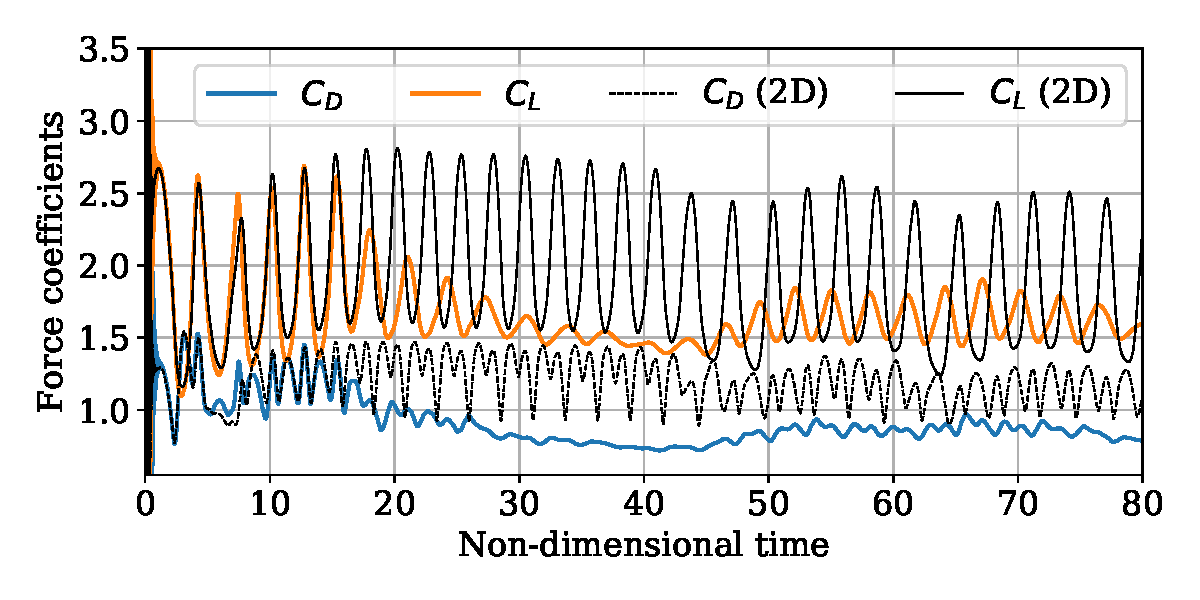
\includegraphics[width=8cm]{figures/forceCoefficientsCompare2D.pdf}
    \caption{History of the force coefficients obtained with two- and three-dimensional simulations at Reynolds number $2000$ for a snake cross-section with a $35$-degree angle of attack.}
    \label{fig:force_coefficients}
\end{figure}

\begin{table*}[!h]
    \renewcommand{\arraystretch}{1.5}
    \caption{Details about the computational grids used for the snake simulations with PetIBM.}
    \label{tab:grid_specs}
    \centering
        \begin{tabular}{clllll}
        Case & Domain & Uniform region & Smallest cell-width & Stretching ratio & Size \\
        \hline
        2D & $30 \times 30$ & $\left[ -0.52, 3.48 \right] \times \left[ -2, 2 \right]$ & $0.004 \times 0.004$ & $1.01$ & $1704 \times 1706$ \\
        3D & $30c \times 30c \times 3.2c$ & $\left[ -0.52, 3.48 \right] \times \left[ -2, 2 \right] \times \left[ 0, 3.2 \right]$ & $0.008 \times 0.008 \times 0.08$ & $1.01$ & $1071 \times 1072 \times 40$ \\
        \hline
    \end{tabular}
\end{table*}

\begin{table}[!h]
    \renewcommand{\arraystretch}{1.5}
    \caption{Time-averaged force coefficients on the snake model at Reynolds number $2000$ and angle of attack $35^o$ for the two- and three-dimensional configurations. (We average the force coefficients between $40$ and $80$ time units of flow simulation and report the relatively difference of the 2D values with respect to the 3D ones.)}
    \label{tab:force_coefficients}
    \centering
    \begin{tabular}{cll}
        Case & $<C_D>$ & $<C_L>$ \\
        \hline
        3D & $0.8390$ & $1.5972$ \\
        2D & $1.1567$ ($+37.9\%$) & $1.8279$ ($+14.4\%$) \\
        \hline
    \end{tabular}
\end{table}

\begin{figure}[!h]
    \centering
    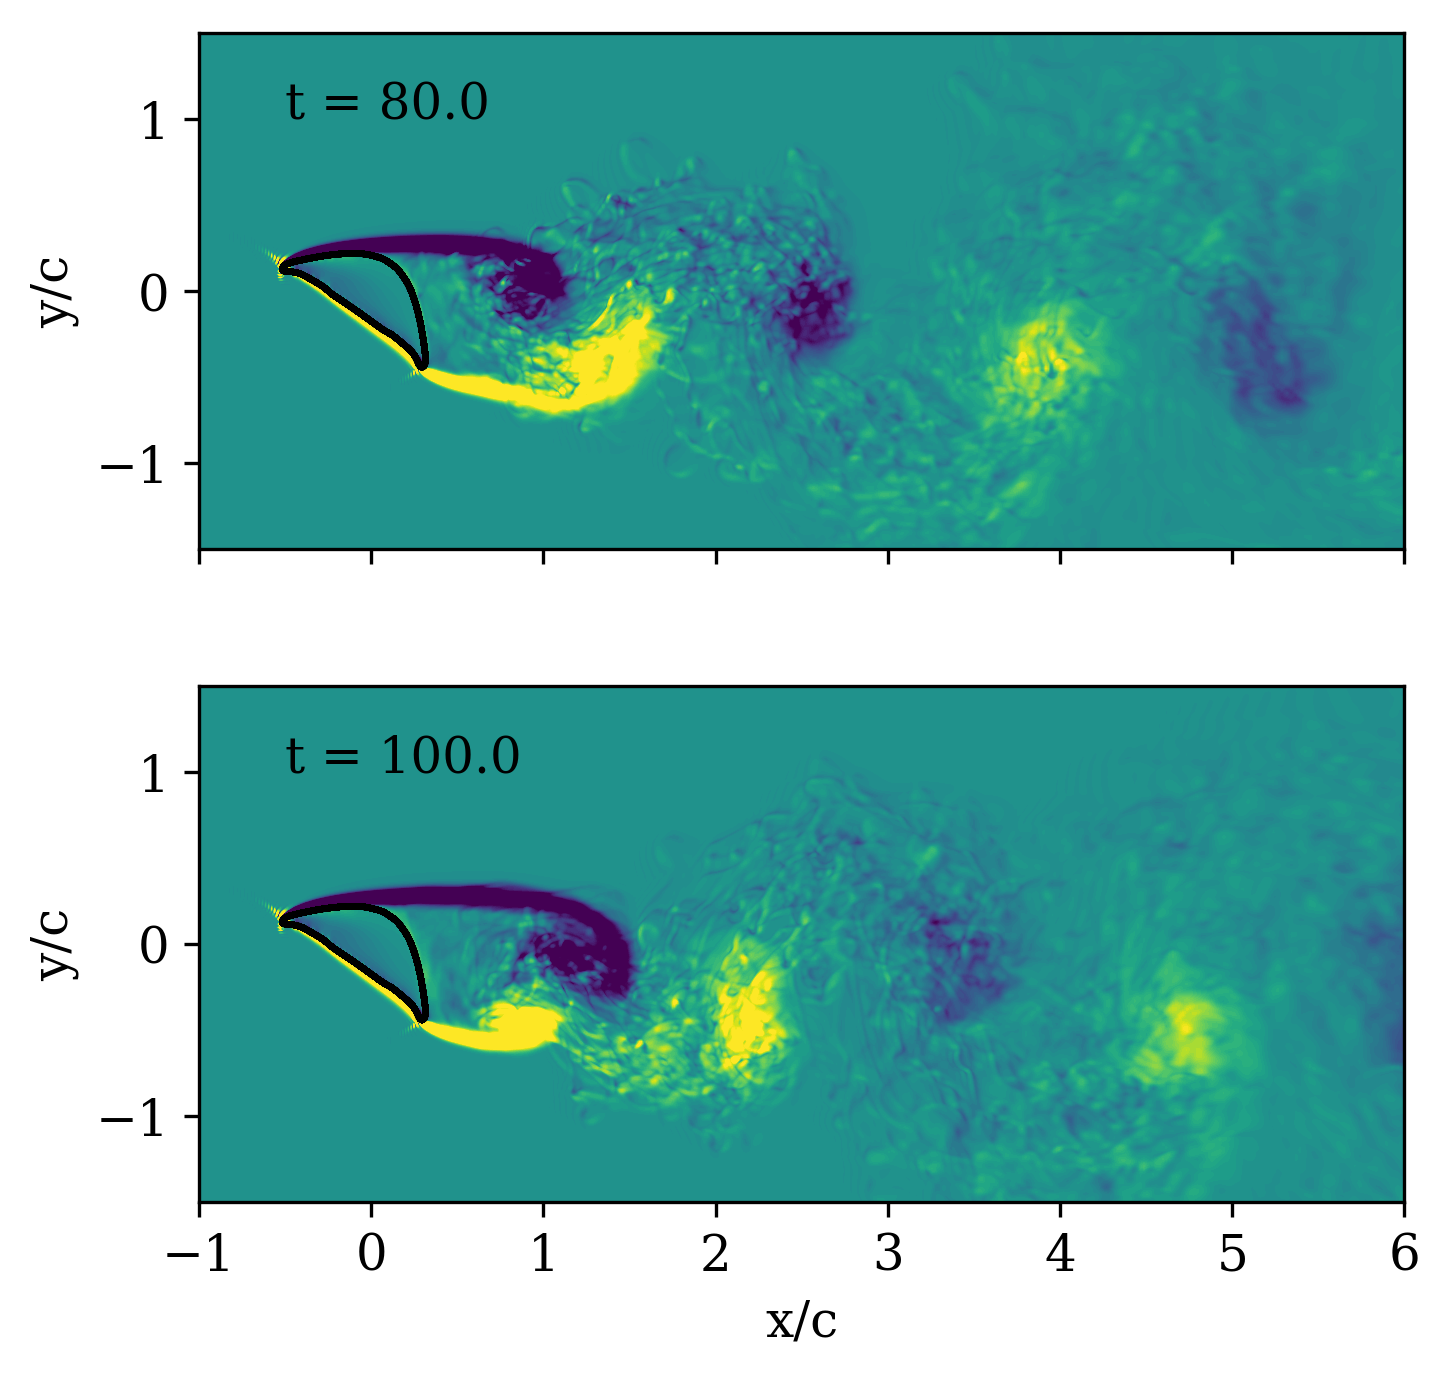
\includegraphics[width=8cm]{figures/wz_avg_multi_contourf.png}
    \caption{Filled contour of the spanwise-averaged z-component of the vorticity ($-5 \leq w_z c / U_\infty \leq 5$) field after $80$ and $100$ time units of flow simulation with PetIBM for the snake cylinder with a cross-section at a $35$-degree angle of attack and Reynolds number $2000$.}
    \label{fig:wz_avg_3d}
\end{figure}

\begin{figure}[!h]
    \centering
    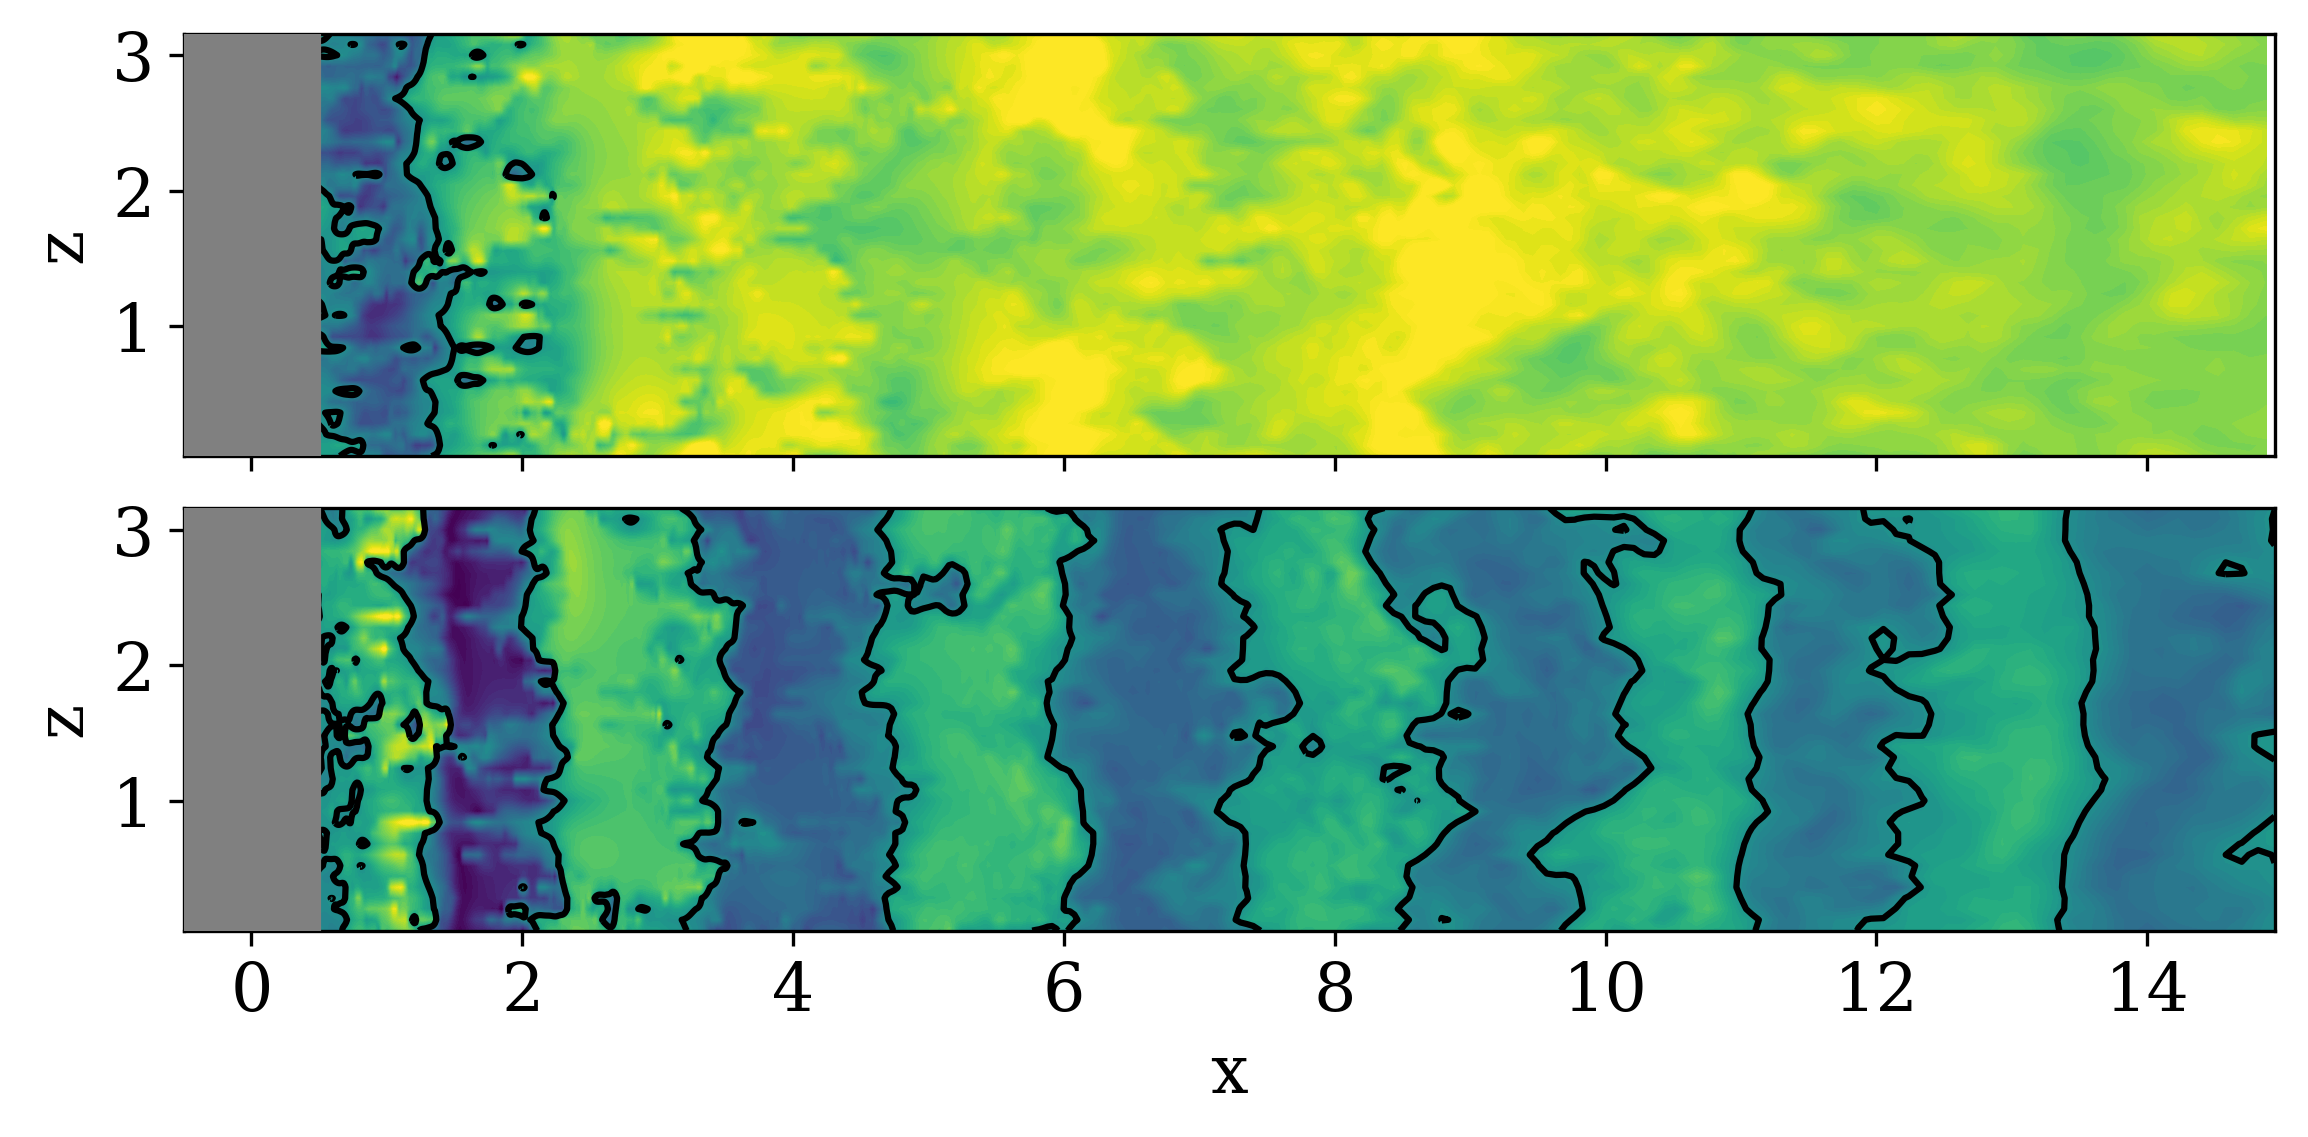
\includegraphics[width=8cm]{figures/ux_uy_xz_plane.png}
    \caption{Filled contour of the streamwise velocity (top) and cross-flow velocity (bottom) behind the snake cylinder in the $x/z$ plane at $y/c=-0.2$ in the wake of the snake cylinder with a $35$-degree angle of attack at Reynolds number $2000$ after $100$ time-units of flow simulations. There are 52 contours from $-1.0$ to $1.0$. The grey area shows a projection of the snake cylinder in the $x/z$ plane. The solid black line defines the contour with $u_x = 0$ (top) and $u_y = 0$ (bottom).}
    \label{fig:ux_uy_xz_plane_3d}
\end{figure}

\begin{figure*}[!h]
    \centering
    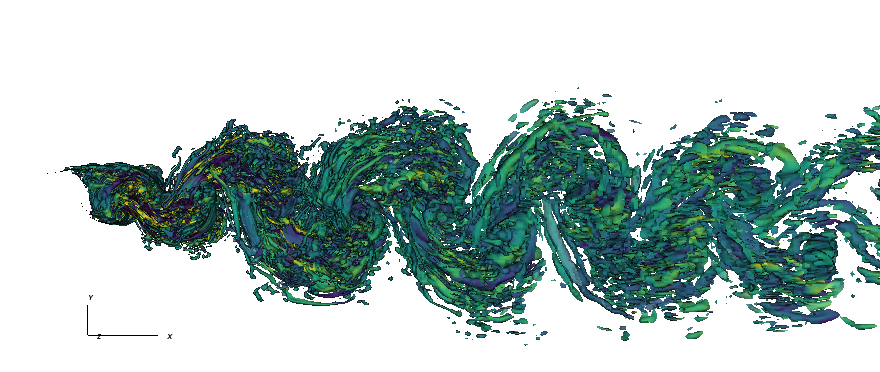
\includegraphics[width=16cm]{figures/qcrit_wx_wake3d_0020.png}
    \caption{Lateral view of the isosurfaces of the Q-criterion ($Q = 1.0$) in the wake of the snake cylinder (with a $35$-degree angle of attack) at Reynolds number $2000$. The isosurfaces are colored with the streamwise vorticity ($-5 \leq w_x c / U_\infty \leq 5$). The figure was generated using the visualization software VisIt \cite{childs_et_al_2012}.}
    \label{fig:qcrit_wx_3d}
\end{figure*}

\section{Cost Analysis and Lessons Learned}\label{sec:cost}

% Mention the 7-day limitation for jobs with Azure Batch. (WARNING: according to the Batch Shipyard documentation, tasks can have a maximum lifetime of 180 days.)
% Mention that Batch Shipyard can pull images from public and private registries.
% Mention that Singularity containers are also supported in Batch Shipyard.

For the year $2018$, Microsoft Azure granted our research lab a sponsorship in terms of cloud credits to run CFD simulations with our in-house software.
We a ``pay-as-you-go'' type of subscription, users can directly sees how much it costs to run a scientific application on a public cloud; such information is often hidden to end-users on university-managed clusters.
From May to December, we spend a total of $20,614$ USD to run simulations of the gliding snake.
During that period, we have been charged data management, networking, storage, bandwidth, and virtual machines (Table \ref{tab:azure_charges}).
More than $99\%$ of the charges are due the usage of virtual machines.
We had the opportunity to use different instances on Microsoft Azure and most the charges for the usage of virtual machines of the \texttt{NC24r} instance (used for the two- and three-dimensional simulations of the flying snake).
The \texttt{NC24r} instance is part of the NC-series (Table \ref{tab:nc_series}); we copiously used as it enables RDMA capabilities for our MPI application and features NVIDIA K80 GPU devices.
For example, the two-dimensional snake run reported in the present article cost $55.4$ USD ($2$ \texttt{NC24r} instances with a hourly price of $3.96$ USD for about $7$ hours).
The three-dimensional computation cost $1077.1$ USD ($2$ \texttt{NC24r} instances for about $136$ hours).

\begin{table}
    \renewcommand{\arraystretch}{1.5}
    \caption{Charges incurred for the usage of different services on Microsoft Azure.}
    \label{tab:azure_charges}
    \centering
    \begin{tabular}{cll}
        Service name & Cost (USD) & \% of total cost \\
        \hline
        Bandwidth & $46.85$ & $0.23$ \\
        Data Management & $0.56$ & $0.003$ \\
        Networking & $1.38$ & $0.007$ \\
        Storage & $25.93$ & $0.16$ \\
        Virtual Machines & $20,582.64$& $99.6$ \\
        \hline
        Total & $20,614$ & \\
        \hline
    \end{tabular}
\end{table}

\begin{table*}[!h]
    \renewcommand{\arraystretch}{1.5}
    \caption{NC series on Microsoft Azure. (Prices as of March 24, 2019, for CentOS or Ubuntu Linux Virtual Machines in the East US region.)}
    \label{tab:nc_series}
    \centering
    \begin{tabular}{cccccccc}
        Instance & cores & RAM & disk sizes & GPU & pay-as-you-go & 1-year reserved & 3-year reserved \\
        && (GiB) & (Gib) && (\$/hr) & (\$/hr) & (\$/hr) \\
        \hline
        NC6 & 6 & 56 & 340 & 1 x K80 & 0.90 & 0.5733 & 0.3996 \\
        NC12 & 12 & 112 & 680 & 2 x K80 & 1.80 & 1.1466 & 0.7991 \\
        NC24 & 24 & 224 & 1,440 & 4 x K80 & 3.60 & 2.2932 & 1.5981 \\
        NC24r\footnotemark & 24 & 224 & 1,440 & 4 x K80 & 3.96 & 2.5224 & 1.7578 \\
        \hline
    \end{tabular}
\end{table*}
\footnotetext{The NC24r configuration provides a low latency, high throughput network interface optimized for tightly coupled parallel applications.}

Running CFD simulations on Microsoft Azure was a first time for our research lab.
As novices in cloud computing, it took us several months to become familiar with the technical vocabulary and the infrastructure of Microsoft Azure before we could submit our first simulation of the snake.

Command-line tools such as Azure-CLI and Batch Shipyard were greatly helpful to create and submit everything from our local terminal. (In our research lab, we tend to avoid, as much as possible, interacting with graphical-user interfaces, so as to make our workflow more reproducible.)
Azure-CLI helped us to setup the Azure Batch account and its associated Azure Storage, as well as uploading/downloading our simulation data.
With Batch Shipyard, users do not need to have experience with the Azure Batch SDK.
We have used Batch Shipyard to submit jobs on Azure Batch to run Docker container-based multi-tasks.
Note that Batch Shipyard also support Singularity containers.

Our in-house CFD research software makes use of the MPI library to run applications on distributed-memory architectures.
We used Azure instances that feature a network interface for remote direct memory access (RDMA) connectivity, allowing nodes in the same pool to communicate over an InfiniBand network.
As of this writing, only Intel MPI 5.x versions are supported with the Azure Linux RDMA drivers.

Moreover, Microsoft Azure implements quotas, such as the maximum number of cores that can be used in a certain region.
To run our simulations, we had to open online customer support requests every time we wanted to increase our core quota for a subscription, with a certain service in certain region with a certain type of instances.
We had to go through this process at least five times during our sponsorship period.

In a new effort to make our research transparent and reproducible by others, we have version-controlled all the input files, pre- and post-processing scripts, as well as the Dockerfiles (used to create the Docker images), the Batch Shipyard configuration files, and command-line instructions required to rerun the simulations on Microsoft Azure.
In addition, all the scripts to reproduce the figures in the present article are made available.
The reproducibility packages are hosted on GitHub in the repository \texttt{cloud-repro}.\footnote{\url{https://github.com/barbagroup/cloud-repro}}

 \section*{Acknowledgment}

This study was possible thanks to a sponsorship from the Microsoft Azure for Research program,\footnote{Microsoft Azure for Research: \url{https://www.microsoft.com/en-us/research/academic-program/microsoft-azure-for-research/}}.

\bibliographystyle{IEEEtran}
% argument is your BibTeX string definitions and bibliography database(s)
\bibliography{IEEEabrv,MesnardoBarba2019}
%
% <OR> manually copy in the resultant .bbl file
%\begin{thebibliography}{1}
%\bibitem
%\end{thebibliography}

\end{document}


